\makeatletter
\def\input@path{{../../}}
\makeatother
\documentclass[../../main.tex]{subfiles}

\graphicspath{
	{../../img/}
	{../img/}
	{img/}
}

\begin{document}
	
	\begin{proof}
		
	Будем использовать формулу \eqref{lec14:15} в предположении, что
	$D$ и $G$ ~--- квадрируемые компакты в $\R^n$. Рассмотрим произвольное 
	разбиение $P =
	\{ D_k \},\; k = \overline{1, m}$ измеримого компакта $D \subset 
	\R^n$ на измеримые компакты $D_k$, так что $D = \bigcup\limits_{k = 1}^{m} 
	D_k$ 
	и $\mes\left(D_i \cap D_j\right) = 0,\; i = j$ т.~е. различные части $D_i$ и 
	$D_j$ могут иметь общими лишь, может быть, граничные точки.
		   
	При диффеоморфизме \eqref{lec14:11} и \eqref{lec14:12} разбиение $P$ 
	множества $D$ порождает соответствующее разбиение измеримого компакта 
	$G \subset \R^n$ на соответствующие измеримые компакты
	$G_k = g(D_k)$, которые являются соответствующими образами обратного 
	диффеоморфизма 
	\eqref{lec14:12} по отношению к \eqref{lec14:11}. При этом так же, как и выше,
	$
	\bigcup\limits_{k = 1}^{m} G_k = G$ и $\mes\left(G_i \cap G_j\right) = 0$, 
	$\forall i \neq j$.
	
	Используя теорему о среднем для $n$-кратного интеграла (формулируется и 
	доказывается аналогично соответствующей теореме для ОИ), 
	в силу интегрируемости имеем:
	
	\[
	\begin{gathered}
	\exists N_k \in G_k,\; k = \overline{1, m} \implies \Delta D_k = \mes D_k 
	= \int\limits_{G_k} |I(t)| dt = \\ = |I(N_k)|
	 \Delta G_k,\; \Delta G_k = \mes G_k = \int\limits_{G_k} dt.
	\end{gathered}
	\]
	
	Полученное таким образом разбиение $\widetilde{P} = \{ G_k  \},\; 
	k = \overline{1, m}$, с множеством отмеченных точек $\widetilde{Q} = \{ N_k \}$
	даёт для разбиения $P = \{D_k\}$ множество отмеченных точек $Q : M_k = 
	f(N_k) 
	\in D_k$. В результате для соответствующей интегральной суммы:
	
	\[
	\begin{cases}
	Q = \{ M_k \},\\
	\widetilde{Q} = \{ N_k \};
	\end{cases}
	\]
	
	\begin{equation}
	\label{lec15:40}
	\begin{gathered}
	\sigma = \sigma \{ h; (\widetilde{P}; \widetilde{Q}) \} = \sum_{k = 1}^{m} h 
	\left( f \left( N_k \right) \right)|I(N_k)| \Delta G_k = \\ = 
	\sigma \{ h; \left( P; Q \right) \} = \sum_{k = 1}^{m} h 
	\left( M_k \right) \Delta D_k.
	\end{gathered}
	\end{equation}
	
	Поэтому, учитывая, что при диффеоморфизме \eqref{lec14:11}, \eqref{lec14:12} 
	имеем $d = \diam P \to 0$ $ \iff \widetilde{d} = \diam \widetilde{P} \to 0$,
	получаем, что, несмотря на использование специальных интегральных сумм, 
	за счёт 
	выбора точки и в силу непрерывности подынтегральной функции  предел общих 
	интегральных сумм будет такой же, как и у специальных, так как непрерывная 
	ФНП 
	является интегрируемой. Поэтому
	
	\begin{equation}
	\label{lec15:41}
	\begin{gathered}
	\int\limits_{D} h \left( x \right) dx = \lim\limits_{d \to 0} \sigma\{ h; 
	\left(P; Q \right)  \} = \lim\limits_{\widetilde{d} \to 0} \sum_{k = 1}^{m} h
	\left( f \left( N_k \right) \right) | I ( N_k ) | \Delta G_k =\\= 
	\left[x = f(t) \right] = \int\limits_{G} | I (t) | h 
	\left( f \left( t \right) \right) dt.
	\end{gathered}
	\end{equation}
	\end{proof}
	
	\begin{iex}
	Пусть $ n = 2 $, то есть имеем плоскость $ \R^2 $, снабжённую 
	ПДСК $ Oxy $. Если используем полярную замену переменных
	\begin{equation}
	\label{lec15:42} 
	\begin{cases}
	x = r\cos\phi,\\
	y = r\sin\phi, 
	\end{cases}
	\end{equation} то для якобиана этой замены имеем
	\[I = \begin{vmatrix}
	x_r' & x_\phi' \\
	y_r' & y_\phi' \\
	\end{vmatrix} = 
	\begin{vmatrix}	
	\cos\phi & -r\sin\phi \\
	\sin\phi & r\cos\phi \\
	\end{vmatrix} = r.\]
	Если в рассмотренной области для $ \left( r, \phi \right) \in G $, 
	являющейся соответствующим образом при отображении \eqref{lec15:42} 
	квадрируемого 
	компакта $ D \subset \R^2$, выполнено $r > 0$, в результате имеем 
	диффеоморфизм \eqref{lec15:42}. В этом случае замена переменной 
	\eqref{lec15:41} даёт:
	\begin{equation} 
	\label{lec15:43}
	\begin{gathered} 
	\iint\limits_{D} h \left( x, y \right) dx dy = \left[ h\left( x, y \right) 
	\text{ непрерывна на } D \subset \R^2 \right] 
	\stackrel{\eqref{lec15:42}}{=}\\= \iint\limits_{G} r f 
	\left( r\cos\phi,\; r\sin\phi \right) dr d\phi.
	\end{gathered}
	\end{equation}
	
	\eqref{lec15:43} остаётся справедливой не только тогда, когда $ r > 0 $, 
	но и $ r \geq 0 $, причём $ r = 0 $ верно лишь на конечном множестве точек.
	\end{iex}
	
	\begin{exmp} (с иллюстрацией)
	
	Рассмотрим $\displaystyle I_0 = \iint\limits_{x^2+y^2 \leq 2x+2y} (x+y)dx 
	dy.$
	
	
	Выделяя полные квадраты, получаем $D: (x - 1) ^ 2 + (y - 1) ^ 2 \leq 2$~--- 
	круг с центром в точке $C_0(1, 1)$ и радиусом $r = \sqrt{2}$.
	
	Геометрически имеем:
	
	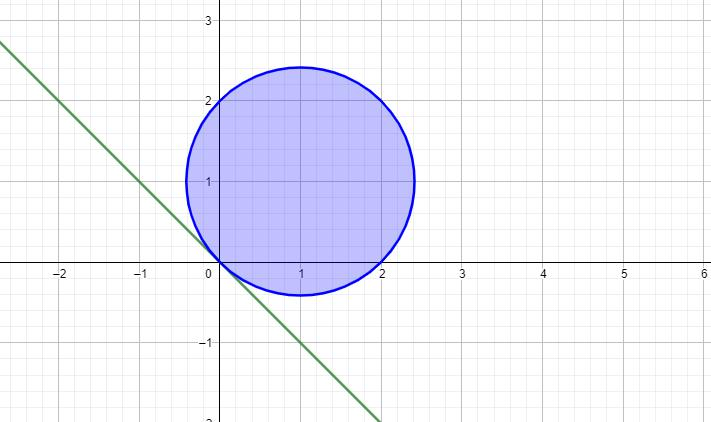
\includegraphics[scale=0.7]{lec15_1}
	
	В данном случае, проводя касательные в точке $(0, 0)$, которые в данном 
	случае сливаются в одну прямую, получаем $-\dfrac{\pi}{4}\leq 
	\phi 
	\leq \dfrac{3\pi}{4},$ $r_1(\phi)=0,$ $r_2(\phi)=2(\cos{\phi} + \sin{\phi}).$
	
	$\displaystyle I_0 = \iint\limits_{G} r(r\cos{\phi}+r\sin{\phi})dr d\phi=
	\int\limits_{-\frac{\pi}{4}}^{\frac{3\pi}{4}}d\phi 
	\int\limits_{0}^{2(\cos{\phi}
	+\sin{\phi})}r^2(\cos{\phi}	+\sin{\phi})dr=\\=	\int\limits_{-\frac{\pi}{4}}^
	{\frac{3\pi}{4}}\left[\frac{r^3}{3}(\cos\phi+\sin\phi)\right]_{r=0}^
	{r=2(\cos{\phi}+\sin{\phi})}d\phi=\frac{8}{3}\int\limits_{-\frac{\pi}{4}}^
	{\frac{3\pi}{4}}(\cos{\phi}+\sin{\phi})^4 d\phi=\frac{8}{3}\int\limits_
	{-\frac{\pi}{4}}^{\frac{3\pi}{4}}(1 +\sin{2\phi})^2 d\phi 
	=\\=\frac{8}{3}\int\limits_{-\frac{\pi}{4}}^
	{\frac{3\pi}{4}}\left(1 +2\sin{2\phi}+\frac{1-\cos{4\phi}}{2}\right)^2 d\phi=
	\frac{8}{3}\left[\frac{3}{2}\phi - \cos{2\phi} - \frac{1}{8}\sin{4\phi}
	\right]_{-\frac{\pi}{4}}^{\frac{3\pi}{4}}=4\pi.$
	\end{exmp}

	\begin{iex}
		Пусть $ n = 3 $, то есть имеем $ \R^3 $, c ДПСК $ Oxyz $. Аналогом полярной 
		замены 
		будут:
		\begin{itemize}
			\item[а)]
			Цилиндрическая замена
			
			\[\begin{cases}
				x = r \cos{\phi},\\
				y = r \sin{\phi},\\
				z = z,
			\end{cases}\]
			т.~е. любой точке $M(x,y,z)$ сопоставляют ее проекцию на плоскость $Oxy$ и 
			производят полярную замену, а $z$ остается собой.
			
			В этом случае якобиан $I = \begin{vmatrix}
			x'_r & x'_\phi & 0 \\
			y'_r & y'_\phi & 0 \\
			0 & 0 & 1
			\end{vmatrix}=r\geq 0$.
			
			В случае $r > 0$ для непрерывной $h=h(x, y, z)$ и соответствующих
			кубируемых компактов в $\R^3$ имеем:
			
			\begin{equation}
			\label{lec15:44}
			\iiint\limits_{D} h(x, y, z) dx dy dz=
			\iiint\limits_{G} rh(r\cos{\phi},\; r\sin{\phi},\; z) dr d\phi dz.
			\end{equation}
			
			\eqref{lec15:44} можно использовать, когда $r=0$ выполнено лишь на конечном 
			множестве  точек, как и в полярной замене.
			\[
			\begin{cases}
			r = [0,\;+\infty], \\ \phi \in [0,\; 2\pi].
			\end{cases}\]\
			На практике иногда удобно рассматривать
			отрицательные углы $(-\pi \leq \phi \leq \pi)$, или брать $\phi$ из
			соответствующих промежутков длины $2\pi$.
			
			\item[б)]
			
			Сферическая замена 
			
			\[\begin{cases}
			x = r \cos{\phi} \cos{\psi},\\
			y = r \sin{\phi} \cos{\psi},\\
			z = r \sin{\psi},
			\end{cases}
			\begin{array}{l}
			 -\frac{\pi}{2}\leq \psi \leq \frac{\pi}{2},\\
			 r \geq 0,\\
			 0 \leq \phi \leq 2\pi.
			\end{array}\]
			
			В данном случае якобиан равен
			\[I = \begin{vmatrix}
				x'_r & x'_\phi & x'_\psi \\
				y'_r & y'_\phi & y'_\psi \\
				z'_r & z'_\phi & z'_\psi
			\end{vmatrix}=r^2\cos{\psi}\geq 0.\]
			
			Поэтому замена переменной для непрерывной $g=g(x, y, z)$ и соответствующих
			кубируемых компактов в $\R^3$ имеет вид:
			\begin{equation}
			\label{lec15:45}
			\iiint\limits_{D} g(x, y, z) dx dy dz=
			\iiint\limits_{G} r^2g(r \cos{\phi} \cos{\psi},\, r \sin{\phi} \cos{\psi},\,
			 r \sin{\psi})\cos{\psi}\, dr d\phi d\psi.
			\end{equation}
		\end{itemize}
	\end{iex}

	\begin{exmp}
		Рассмотрим шар
		\[x^2 + y^2 + z^2 \geq R^2.\]
		После полярной замены имеем \[r^2 \leq R^2, \;\; 0 \leq \phi \leq 2\pi, 
		\;\; -\dfrac{\pi}{2} \leq \psi \leq \dfrac{\pi}{2}.\]
		
		Для объема шара имеем
		\[V_{\text{ш}} = \iiint\limits_{x^2 + y^2 + z^2 \leq R^2} dxdydz = 
		\iiint\limits_{
			\substack{
			r \leq R\\
			0 \leq \phi \leq 2\pi\\
			-\frac{\pi}{2} \leq \psi \leq \frac{\pi}{2}
			}
		}r^2\cos \phi \; dr d\phi d\psi = \int\limits_{0}^{R}r^2dr\int\limits_{0}^
	{2\pi}\cos\phi \; d\phi \int\limits_{-\frac{\pi}{2}}^{\frac{\pi}{2}}d\psi\]
		
		Переменные полностью разделились, поэтому 3И можно рассматривать как 
		произведение
		 однократных интегралов
		\[
		\left[\dfrac{r^3}{3}\right]_{0}^{R} \cdot \Big[\sin \psi 
		\Big]_{-\frac{\pi}{2}}^{\frac{\pi}{2}} \cdot \Big[\phi\Big]_{0}^{2\pi} = 
		\dfrac{4}{3} \pi R^3 
		\]
	\end{exmp}
	
	Рассмотрим вычисление 2И и 3И с помощью соответствующих общих замен 
	переменных. 
	
	\begin{examples}
~

		\begin{enumerate}
			\item
			Вычислим 2И $\displaystyle I_0 = \iint\limits_D xy\; dxdy$, гдe
			$D: \left[
			\begin{array}{l} 
			xy= 1,\\
			xy = 4,\\
			y = \dfrac{x}{4},\\
			y = 4x,\\
			x \geq 0.
			\end{array}
			\right.
			$
			
			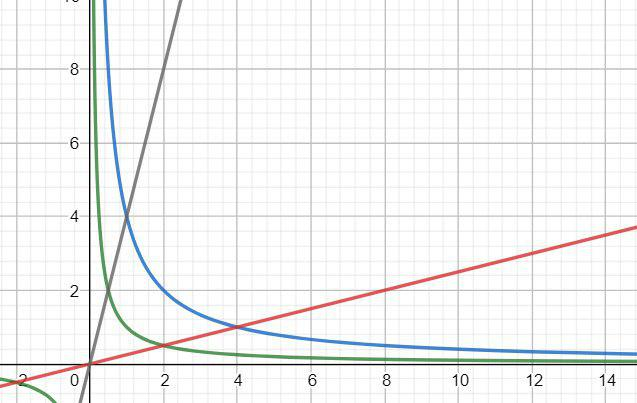
\includegraphics[scale=0.85]{lec15_2}
			
			Воспользуемся общей заменой вида
			\[\begin{cases}
			\smallskip
			u = xy \big|_{1}^{4}\\
			v = \frac{y}{x} \big|_{\frac{1}{4}}^{4}
			\end{cases}\]
			
			Для обратного якобиана получаем: 
			\[J = \begin{bmatrix}
			u'_x & u'_y\\
			v'_x & 	v'_y
			\end{bmatrix} = \begin{bmatrix}
			\smallskip
			x & y\\
			-\frac{y}{x^2}& \frac{1}{x}
			\end{bmatrix} = 2 \dfrac{y}{x} = 2 v > 0.\]
			
			Для прямого якобиана имеем $I = \dfrac{1}{J} = \dfrac{1}{2v}$.
			
			$\displaystyle I_0 = \iint\limits_{\substack{
				1 \leq u \leq 4\\
				\frac{1}{4} \leq v \leq 4
				}} u \cdot \dfrac{1}{2v} \; du 
			dv = \dfrac{1}{2}\int\limits_{1}^{4} u du 
			\int\limits_{\frac{1}{4}}^{4} \dfrac{dv}{v} =
			 \dfrac{1}{2} \left[\dfrac{u ^ 2}{2}\right]_1^4 \cdot 
			 \big[ \ln{v}\big]_{\frac{1}{4}}^4 = 2^3 \ln{4} = 16 \ln{2}.$
			 
			\item Рассмотрим тело, ограниченное поверхностью второго порядка
			
			\[(x + y + z)^2 + (x + y - z)^2 + (x - y + z)^2 \leq 1.\]
			
			Полагая
			\[\begin{cases}
			u = x + y + z,\\
			v =  x + y - z,\\
			w = x - y + z,\\
			\end{cases}\]
			получаем, что образом этого тела является шар $u^2 + v^2 + w^2 \leq 1$.
			
			Для обратного якобиана рассмотренного диффеоморфизма имеем
			
			\[J = \begin{vmatrix}
			u'_x & u'_y & u'_z\\
			v'_x & v'_y & v'_z\\
			w'_x & w'_y & w'_x
			\end{vmatrix} =\begin{vmatrix}
			1 & 1 & 1\\
			1 & 1 & -1\\
			1 & -1 & 1
			\end{vmatrix} = \begin{vmatrix}
			1 & 1 & 1\\
			0 & 0 & 2\\
			0 & 2 & 0
			\end{vmatrix} = -4 < 0 \implies |I| = \frac{1}{4},\]
			поэтому объем будет равен
			\[V = \displaystyle \iiint\limits_{u^2 + v^2 +
				 w^2 \leq 1} \frac{1}{4} d u d v d w
			  = \frac{1}{4} V_{\text{шара}} = \frac{1}{4} \cdot \frac{4}{3}\pi 
			  = \frac{\pi}{3}.\]
		\end{enumerate}
	\end{examples}
\end{document}
